\documentclass{beamer}
\usepackage{minted}
\usepackage{verbatim,color}
\usepackage{hyperref}
\usepackage{graphicx}
\hypersetup{
    colorlinks=true,
    urlcolor=blue,
}

\title{Android Root Detection Evasion}
\author[]{Roberto Castellotti\\{\small Supervised by: prof. Giovanni Lagorio}}
\institute{Università degli Studi di Genova}
\date{2022}

\begin{document}
\makeatletter

\frame{\titlepage}

\begin{frame}{Introduction to Android}

\begin{itemize}
    \item introduzione android
    \item introduzione "apk" https://developer.android.com/guide/components/fundamentals mobisec native code
    \item spiegare come si passa da sorgente java a bytecode
    \item setup root phone (lineage, magisk, twrp, tool vari)
    \item root: perche' farlo
    \item root detection: perche'
    \item root detection: come https://github.com/scottyab/rootbeer
    \item approfondimento signature app (in particolare patchare con frida meglio perche' firma vera)
    \item tool usati
\end{itemize}

\end{frame}


\begin{frame}{patch-and-reinstall}

    \begin{itemize}
        \item {\footnotesize \texttt{adb pull /data/com/app/com.package.name app.apk}}
        \item {\footnotesize \texttt{apktool d app.apk -output app}}
        \item patch
        \item {\footnotesize \texttt{apktool b app -output rebuilt-app.apk}}
        \item {\footnotesize \texttt{zipalign -f -p 4 rebuilt-app.apk  aligned-rebuilt-app.apk}}
        \item {\footnotesize \texttt{apksigner sign --ks ~/key.jks  aligned-rebuilt-app.apk}}
        \item {\footnotesize \texttt{adb install aligned-rebuilt-app.apk}}
        % well technically "this" approach needs it in order to pull the apk, but we can still obtain the apk using com.aurora.store
        \item this approach does not require the android device to be rooted 
    \end{itemize}

\end{frame}

\begin{frame}[fragile]{patch-and-reinstall: an example}

   The patching process is usually a matter of finding the methods performing root detection and patching them, here is an example from a popular financial services company's application:

\begin{figure}
    \centering 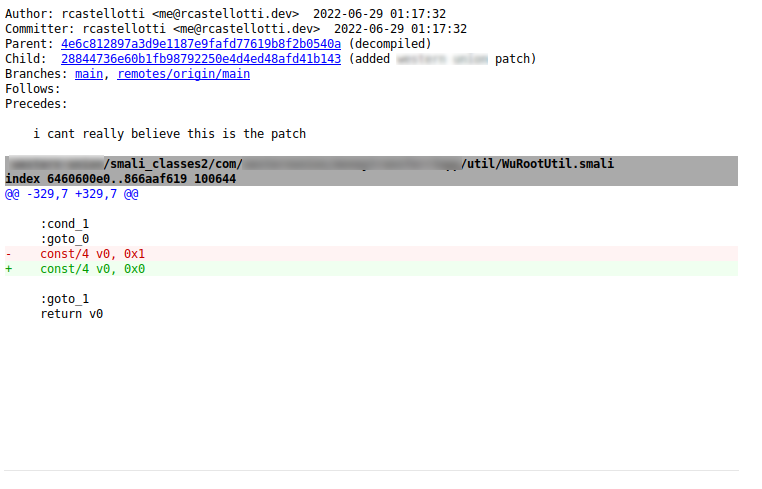
\includegraphics[scale=1.4]{patch.png}
    \caption{patching \mintinline{smali}{.method public static isDeviceRooted()Z} }
\end{figure}

\end{frame}


\begin{frame}{frida: a dynamic toolkit} 

    \begin{itemize}
        \item provides ability to inject scripts into black box processes.
        \item portable (Windows, macOS, GNU/Linux, iOS, Android)
        \item \textbf{injected mode}: \texttt{frida-server}: \texttt{frida-core} over TCP
        \item \texttt{frida-core}: a layer that packages up GumJS into a shared library that it injects into existing software, and provides a two-way communication channel for talking to your scripts.
        \item \textbf{on device:} {\footnotesize \texttt{./frida-server-15.1.27-android-arm64}}
        \item \textbf{on computer:} {\footnotesize \texttt{frida -U -l script.js -f com.package.name}}
        \item this approach could be better since it allows to patch applications without losing original package signature
    \end{itemize}
    
\end{frame}

\begin{frame}{tools used}

    \begin{itemize}
        \item \href{https://developer.android.com/studio}{Android Studio}
        \item \href{https://github.com/iBotPeaches/Apktool}{iBotPeaches/Apktool}:
        A tool for reverse engineering Android apk files
        \item \href{https://github.com/skylot/jadx}{skylot/jadx}: Dex to Java decompiler
        \item \href{https://github.com/scottyab/rootbeer}{scottyab/rootbeer}: Simple to use root checking Android library and sample app
    \end{itemize}
    
\end{frame}

\end{document}